\documentclass[fleqn, xcolor=x11names]{beamer}
\usetheme{Ann}
\usecolortheme{default}

\usepackage[utf8]{inputenc}
\usepackage[T2A]{fontenc}
\usepackage[russian]{babel}
\usepackage{amsmath}
\usepackage{amsfonts}
%\usepackage{amssymb}
\usepackage{hyperref}


\usepackage{graphics, graphicx}
\usepackage{color}
\usepackage{enumerate}

\usepackage{epigraph}
\usepackage{makecell}

\usepackage{tikz}
\usetikzlibrary{patterns}

\usepackage{minted}
\usemintedstyle{default}
%my package
\graphicspath{{../figures/}}
\setbeamertemplate{bibliography item}{\insertbiblabel}

\beamertemplatenavigationsymbolsempty

\setbeamertemplate{itemize item}[ball]
\setbeamertemplate{itemize subitem}[ball]
\definecolor{my_blue}{RGB}{0, 0, 100}


%\usefonttheme[onlylarge]{structurebold} % названия и текст в колонтитулах выводится полужирным шрифтом.
\usefonttheme[onlymath]{serif}  % привычный шрифт для математических формул
%\setbeamerfont*{frametitle}{size=\normalsize,series=\bfseries} % шрифт заголовков слайдов
\usepackage[nopar]{lipsum} %для генерации большого текста

\newminted[pcode]{python}{baselinestretch=1, fontsize=\small}
\newmintinline[pinline]{python3}{baselinestretch=1}
%\definecolor{bg}{rgb}{0.95,0.95,0.95}
%\newminted[lcode]{latex}{baselinestretch=1, bgcolor=bg}
\newmintinline[linline]{latex}{baselinestretch=1}

\usepackage{tcolorbox}
\tcbuselibrary{minted,skins}

\newtcblisting{lcode}{
    listing engine=minted, %use minted for highlight
    colback=lcodebg, %background color
    colframe=black!50, %width of frame
    listing only,
    minted style=colorful,
    minted language=latex,
    minted options={linenos=false,texcl=true}, %lines - number of lines
    left=1mm,
}
\definecolor{lcodebg}{rgb}{0.95,0.95,0.95}

\usepackage{tikz}
\usetikzlibrary{arrows,positioning}
\usepackage{listings}
\lstset{language=Python}

\newcommand{\real}{\mathbb{R}}
\newcommand{\norm}{\mathop{\rm norm}\limits}
\newcommand{\softmax}{\mathop{\rm softmax}\limits}
\newcommand{\argmin}{\mathop{\rm argmin}\limits}

\definecolor{beamer@blendedblue}{rgb}{0.037,0.366,0.75}

\title{\bfseries Интерпретируемое машинное обучение}
\author[Тыцкий В.И.]{Студент: Тыцкий В.И. \\[1ex]  {\small Научный руководитель: Майсурадзе А.И.}}
\institute[ВМК МГУ]{МГУ имени М. В. Ломоносова, факультет ВМК, кафедра ММП}
\date{}

\begin{document}

\begin{frame}
    \titlepage
\end{frame}

\begin{frame}{Оглавление}
     \tableofcontents
\end{frame}


\section{Зачем нужна интерпретация?}

\begin{frame}{Данные $\Rightarrow$ Модель $\Rightarrow$ Done?}
    \centering
    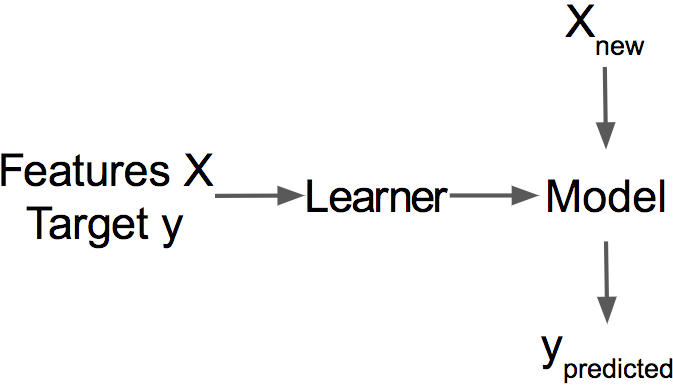
\includegraphics[width=6cm]{explain_pipline_0.png}

    \begin{itemize}
        \item  Постановка задачи 
        \item Определились, что будем решать с помощью ML
        \item Сбор данных
        \item Обучили модель, она работает ''хорошо''
        \item На этом можно остановиться?
    \end{itemize}
    
\end{frame}

\begin{frame}{Проблема черного ящика}
    \centering
    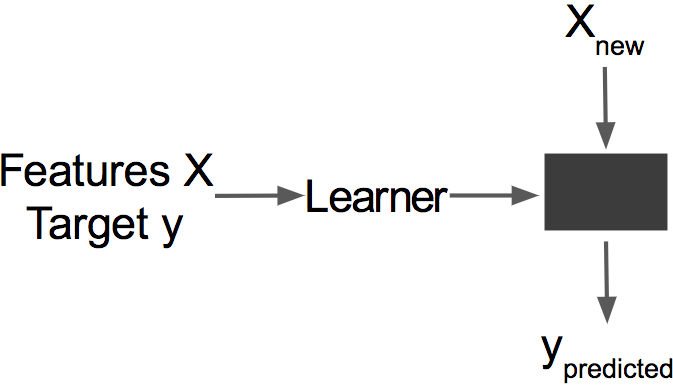
\includegraphics[width=6cm]{explain_pipline_1.png}

    \begin{itemize}
        \item Сбор данных и постановка задачи 
        \item Определились, что будем решать с помощью ML
        \item Обучили модель, она работает ''хорошо''
        \item \textbf{Вместо модели получили ''умный'' черный ящик}
    \end{itemize}
    
\end{frame}

\begin{frame}{Почему мы можем тебе верить?}
    \centering
    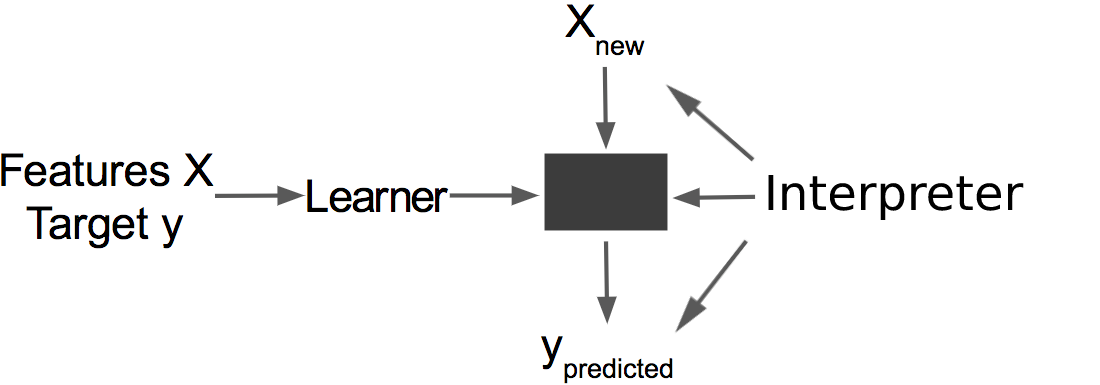
\includegraphics[width=10cm]{interpreter.png}
    \begin{itemize}
        \item Почему модель приняла именно такое решение?
        \item На что модель обращает внимание?
        \item Какие свойства объекта наиболее важны в общем и в совокупности
    \end{itemize}
    
\end{frame}

\begin{frame}{Хорошего качества недостаточно}
    \begin{itemize}
        \item Использование ML несет за собой большие риски:
        \begin{itemize}
            \item Медицина 
            \item Государственные структуры
            \item Банки
        \end{itemize}

        \item Глубже понимаем наблюдаемое явление 
        \item Новые закономерности в данных
        \item Уверенность в адекватности модели
    \end{itemize}
    
\end{frame}

\section{Методы}

\begin{frame}{Классификация методов интерпретации}
    \begin{itemize}
        \item Локальные -- объясняют модель на конкретном объекте
        \item Глобальные -- объясняют как модель работает в целом
        \vspace{10pt}
        \item Специфичные для модели (Model Specific) 
        \item Индифферентные к модели (Model Agnostic)
    \end{itemize}
\end{frame}

\begin{frame}{Model $=$ Interpreter}
    \begin{itemize}
        \item Используем простые модели: линейные, деревья
        \item Структура построения алгоритма сообщает принцип принятия решений
        \item Недостаток: не всегда справляются с задачей
    \end{itemize}
    
\end{frame}

\begin{frame}{Model $=$ Interpreter}

    \begin{columns}
        \begin{column}{0.5\textwidth}
            В случае линейных моделей можем
            посмотреть на вес для каждого признака
            $$y_i = f(<\vec{w}, \vec{x_i}>)$$
        \end{column}
        \begin{column}{0.5\textwidth}  %%<--- here
            В случае решающего дерева
            \centering
            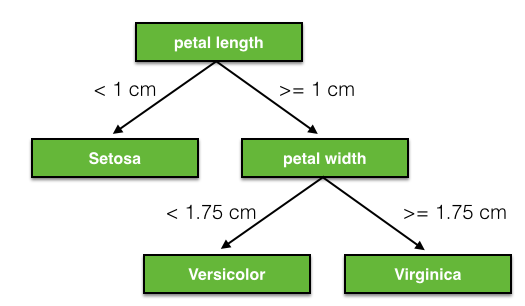
\includegraphics[width=6cm]{decision_tree_0.png}
        \end{column}
    \end{columns}

\end{frame}

\begin{frame}{LIME (Local interpretable model-agnostic explanations)}
    \begin{itemize}
        \item $x$ - конкретный объект
        \item $f$ - черный ящик (мы умеем $x\rightarrow f(x) \rightarrow y$)
        \item $g$ - простая модель (например линейная)
        \item $\pi_x$ - насколько сильно учитываем контекст вокруг 
        \item $\Omega(g)$ - мера сложности модели g
    \end{itemize}

    $$interpreter(x) = \argmin_{g}L(f,g,\pi_x) + \Omega (g)$$
    
\end{frame}

\begin{frame}{LIME}

    $$interpreter(x) = \argmin_{g}L(f,g,\pi_x) + \Omega (g)$$
    $$L(f,g,\pi_x) = \sum\limits_{x'} (f(x') - g(x'))^2\pi_x(x,x')$$

\end{frame}


\begin{frame}{Объясняем объясняющего}
    \centering
    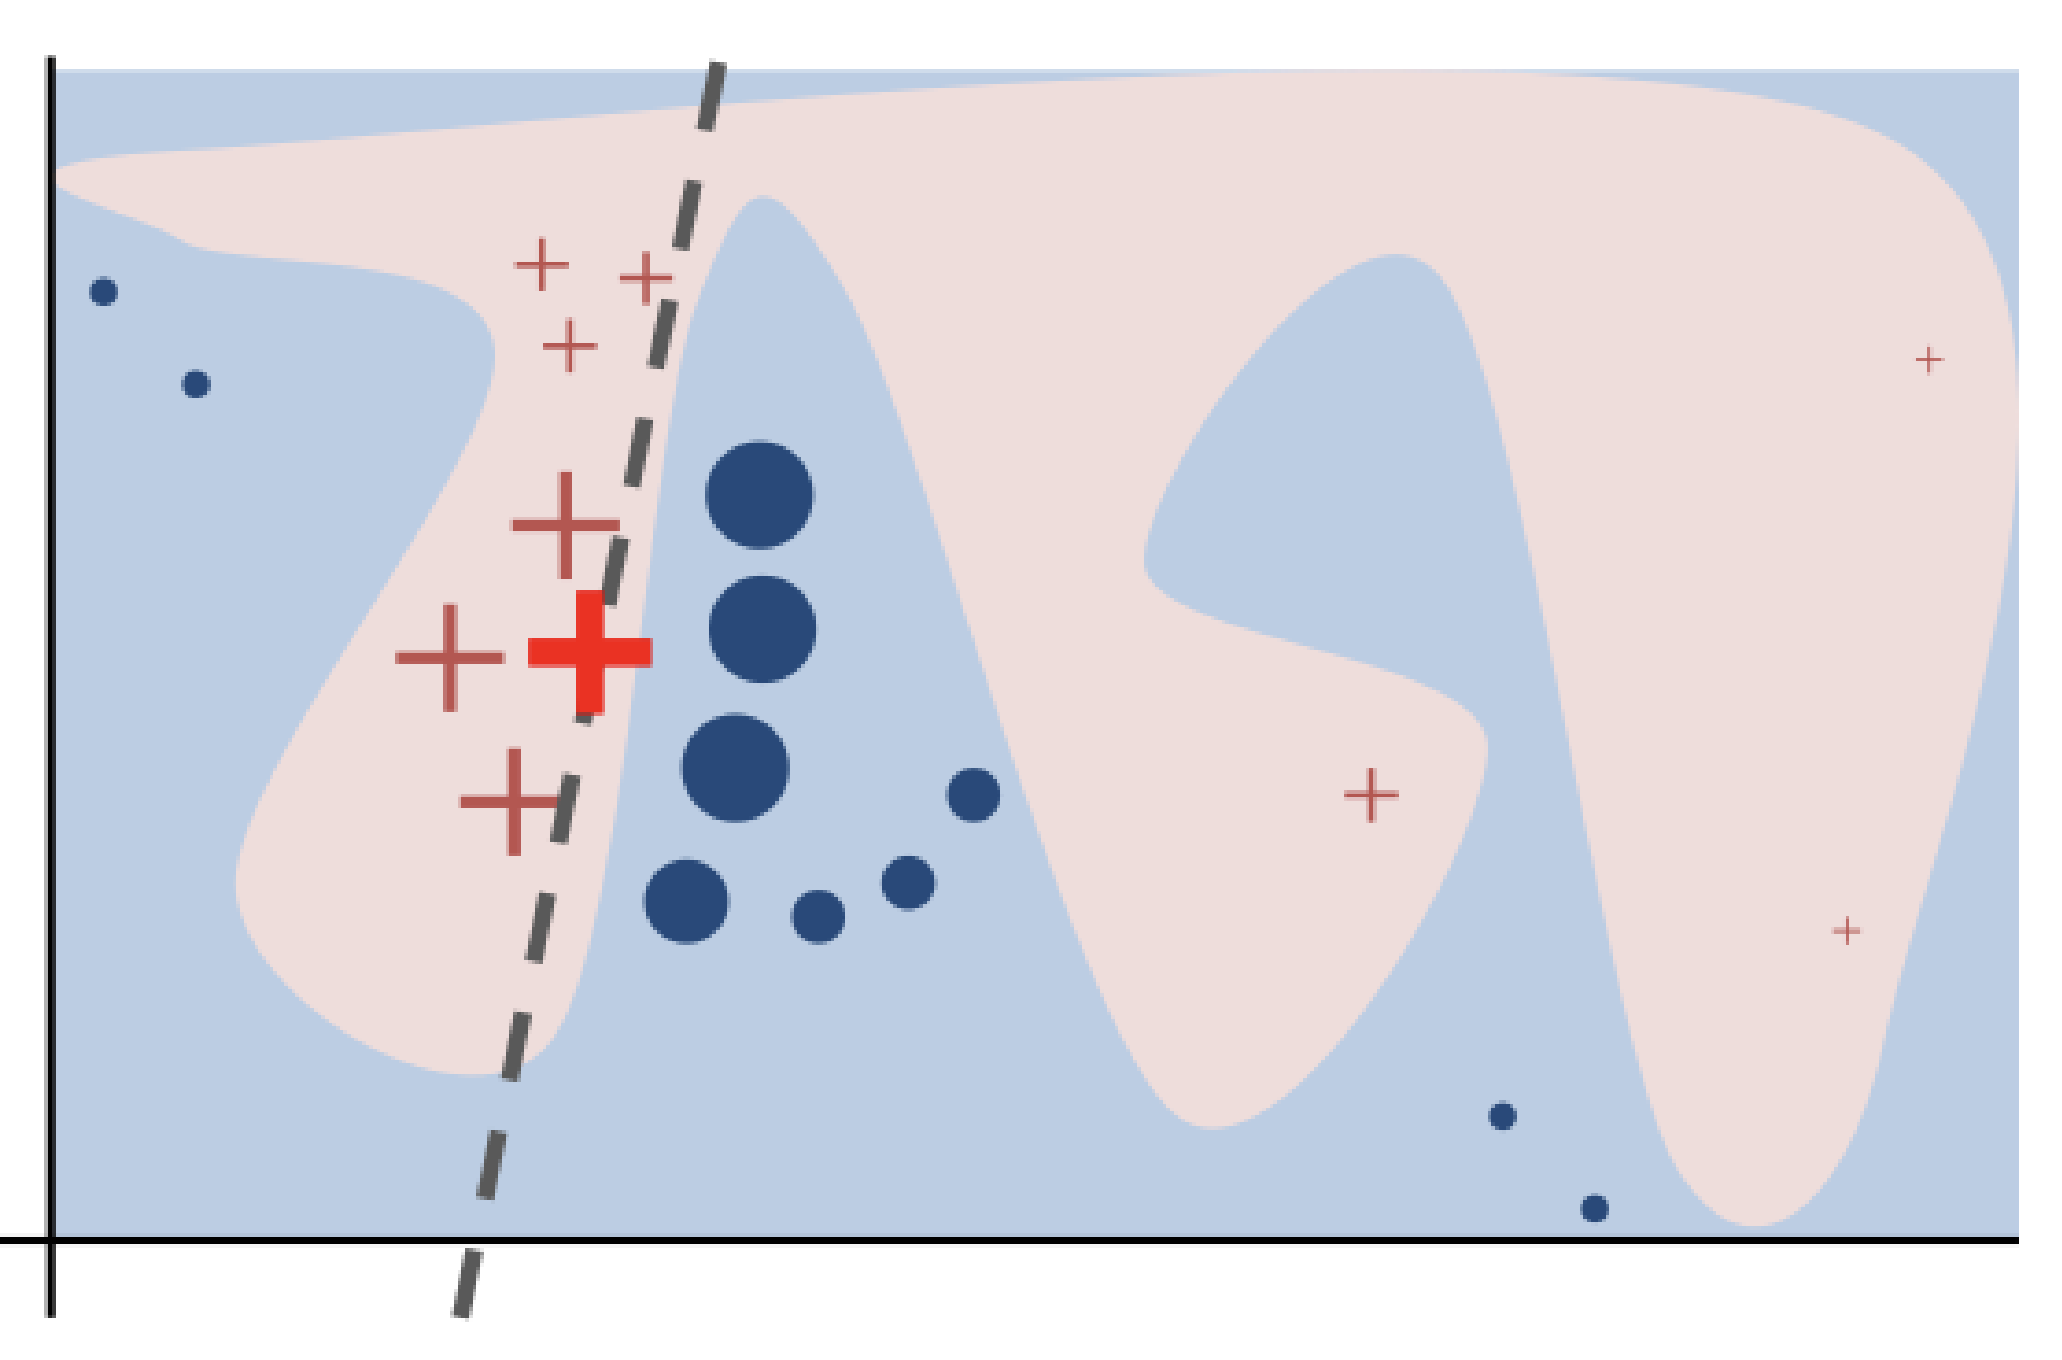
\includegraphics[width=6.5cm]{lime_from_article.png}
    \begin{enumerate}
        \item В качестве простой модели возьмем \textbf{взвешенную} линейную
        \item Выберем объект, который хотим проанализировать
        \item Обучаем линейную регрессию в окрестности объекта
        \item Интерпретируем линейную регрессию!
    \end{enumerate}
\end{frame}

\begin{frame}{Изображения}
    \centering
    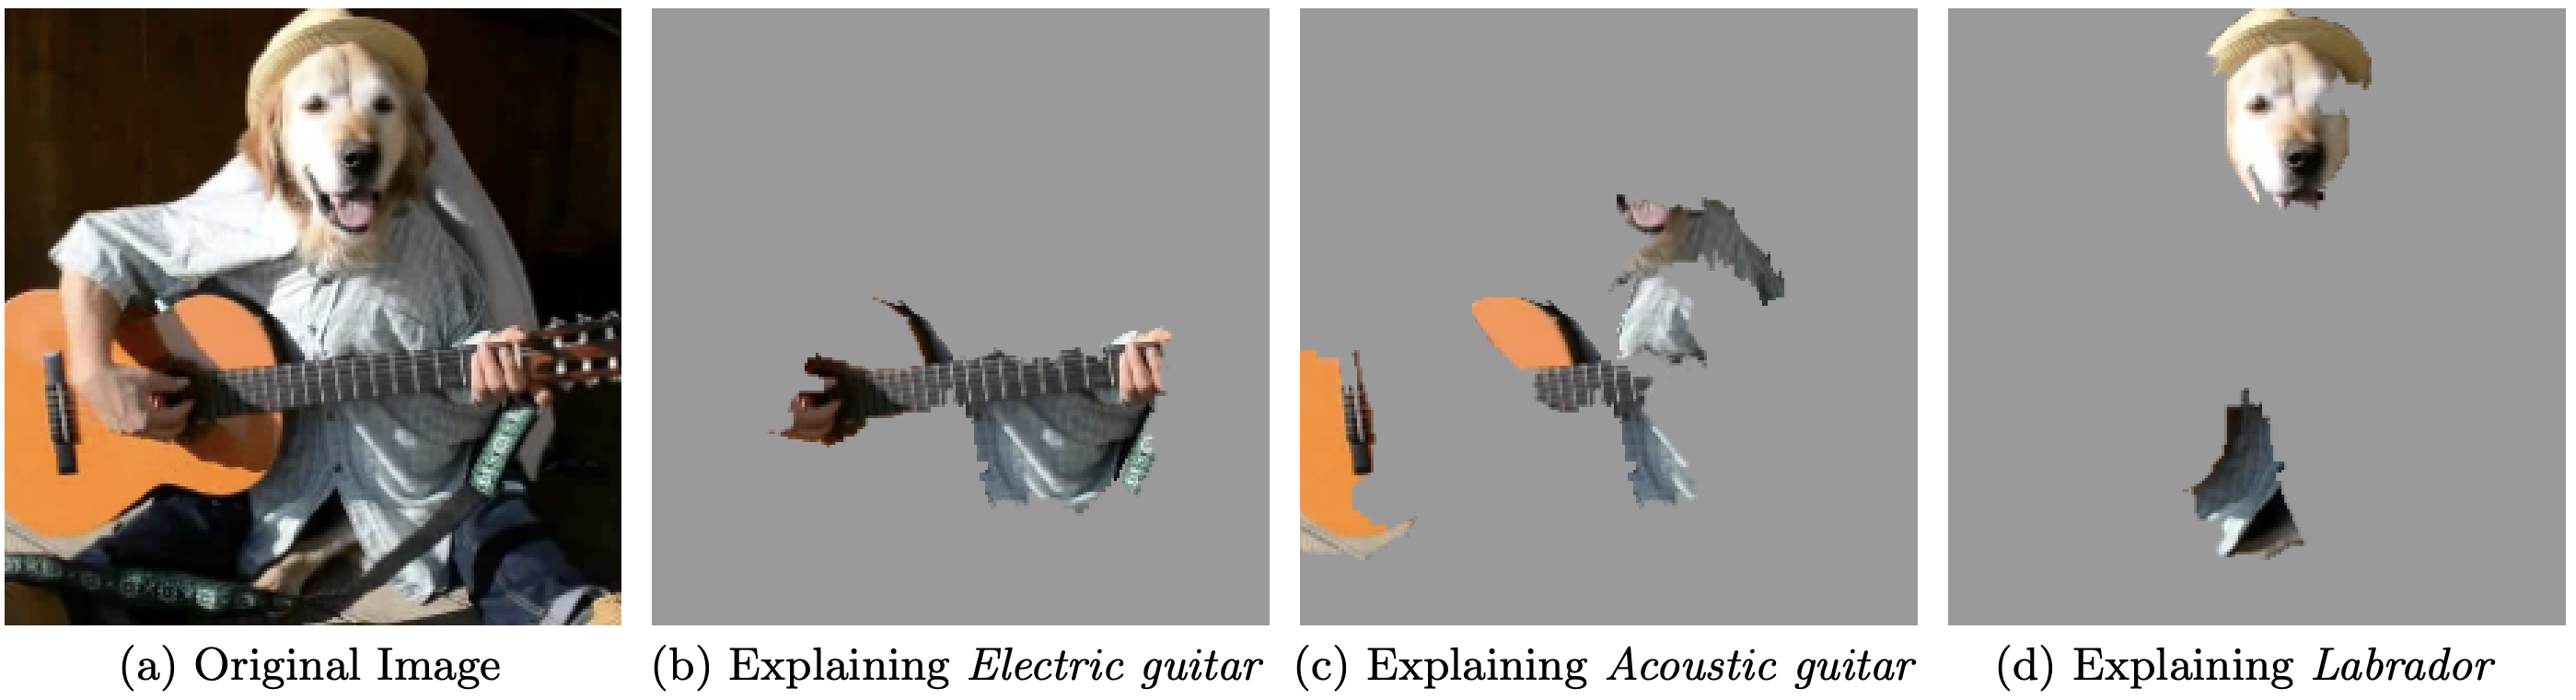
\includegraphics[width=1\linewidth]{good_boy_with_guitar.png}
    \begin{itemize}
        \item Для изображений сложно сказать, что такое окрестность
        \item Будем находить суперпиксели и менять их
        % \item На вход линейной регрессии подается не изображение, 
        % а вектор включений суперпикселей
    \end{itemize}
\end{frame}

\begin{frame}{Shapley values}
    \begin{itemize}
        \item Концепция из кооперативной теории игр
        \item Считаем, что награда пропорциональна вкладу игрока 
        % \item \textbf{При подсчете важен порядок игроков!}
    \end{itemize}

    \vspace{10pt}

    $P$ -- все игроки, $R$ -- всевозможные перестановки игроков

    $u(K)$ -- награда множества игроков K

    $P_i^R$ -- игроки, встретившиеся в перестановке R до i-ого игрока

    $$\phi_i(u) = \frac{1}{N!}\sum\limits_{R}\left[u(P_i^R \cup \{i\}) - u(P_i^R)\right]$$
\end{frame}

\begin{frame}{Shapley values}
    \begin{itemize}
        \item Линейность -- $\phi_i(u+v) = \phi_i(u) + \phi_i(v)$
        \item Симметричность -- награда игрока не зависит от его номера
        \item Аксиома Болвана -- бесполезный игрок не вносит вклад в коалицию
        \item Эффективность -- $\sum\limits_i\phi_i(u) = u(P)$
    \end{itemize}
    $$\phi_i(u) = \frac{1}{N!}\sum\limits_{S \subseteq  P \backslash \{i\}}\frac{1}{C_{N}^{|S|}}\left[u(S \cup \{i\}) - u(S)\right]$$
\end{frame}

\begin{frame}{SHAP\footnote{Некоторые теоретические моменты опущены}}
    Игрок $\rightarrow$ признак

    Награда $\rightarrow$ значение $f(x)$

    \vspace{10pt}

    \begin{itemize}
        \item Выбираем $x \in R^D$
        \item Семплируем ''подмножества признаков'' $z'_{k} \in \{0,1\}^D, k \in \{1,\dots,K\}$
        \item Для каждого $z'_{k}$ \textbf{восстанавливаем} $z_k = h_x(z'_k)$ и находим $f(h_x(z'_k))$
        \item Считаем веса для каждого $z'_{k}$ и обучаем линейную модель
        \item Веса линейной модели будут обладать свойствами shapley values
    \end{itemize}

\end{frame}

\begin{frame}{SHAP}
    

    \begin{itemize}
        \item Операция восстановления $h_x:\{0,1\}^D \rightarrow R^D$ ''заменяет'' 0 на случайное значение
        признака из набора данных, а 1 на значение признака у рассматриваемого $x$
        \item Вес для $z_i'$ считаем по следующей формуле:
        $$\pi_x(z') = \frac{(M-1)}{C_{D}^{|z'|}(M-|z'|)|z'|}$$
    \end{itemize}


\end{frame}

\begin{frame}{SHAP}
    
    
    \centering
    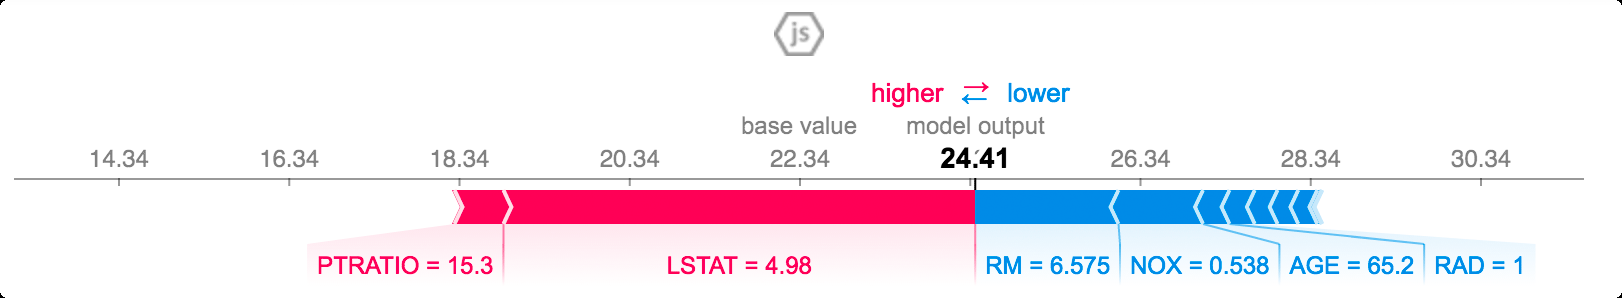
\includegraphics[width=10cm]{single_shap.png}
    \centering
    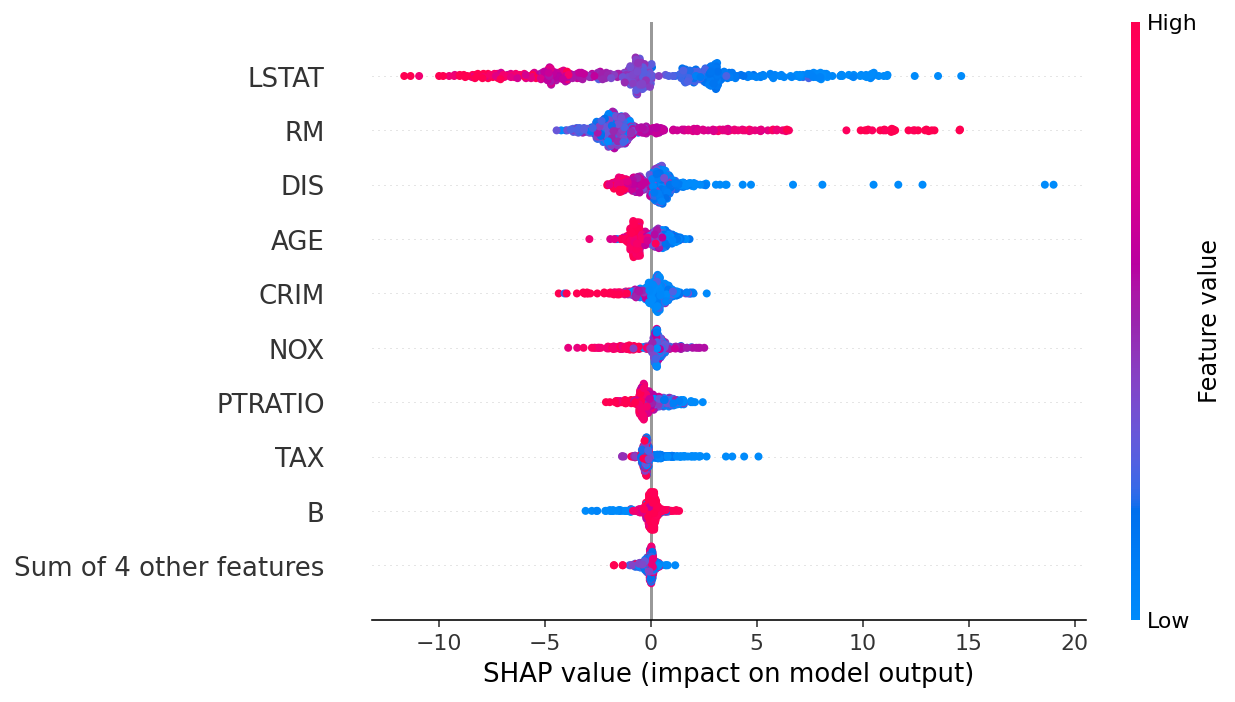
\includegraphics[width=5cm]{summary_shap_0.png}
    \centering
    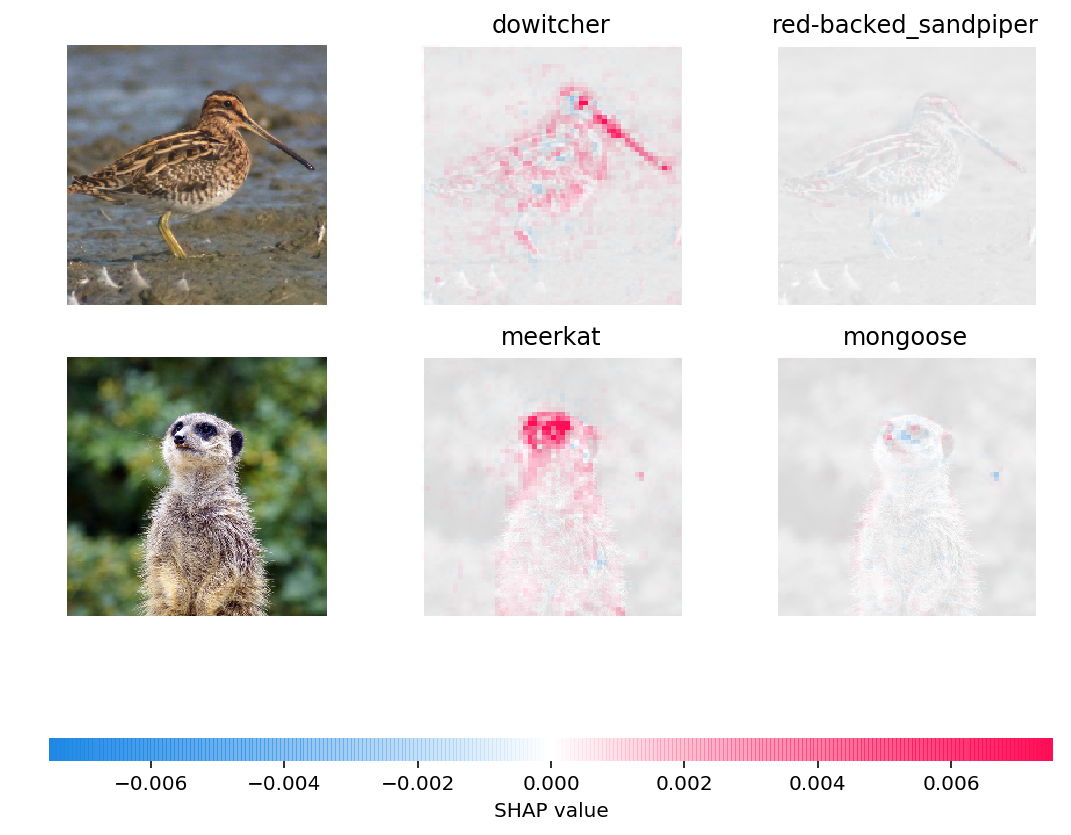
\includegraphics[width=5cm]{images_shap_0.png}


\end{frame}



\section{Применение к временным рядам}

\begin{frame}{Проблемы временных рядов для интерпретации}

    \begin{itemize}
        \item Длина последовательности бывает разной
        \item Огромная размерность пространства 
        \item Один timestamp редко несет в себе много информации
        \item Чем больше признаковое пространство, тем сложнее разобраться
    \end{itemize}

\end{frame}

\begin{frame}{Задачи seq2seq}

    \begin{itemize}
        \item Пусть дана задача seq2seq (открыты ли глаза у человека в конкретный момент)
        \item Для простоты будем считать, что каждый промежутки времени независимы между собой
        \item Обучим модель
        \item Попробуем применить один из методов объяснения модели
    \end{itemize}

\end{frame}

\begin{frame}{Задачи seq2seq}

    \centering
    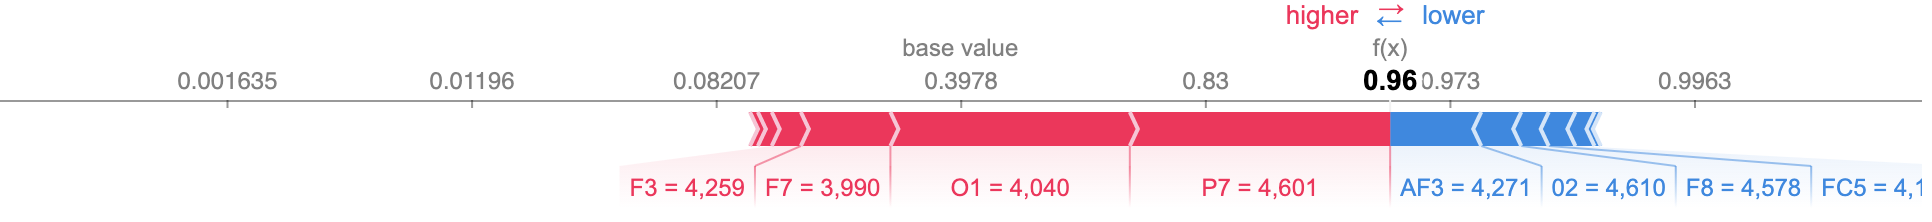
\includegraphics[width=\linewidth]{shap_timestamp.png}

    \vspace{20pt}

    \begin{itemize}
        \item $\text{Accuracy} = 0.88, \quad \text{AUC-ROC} = 0.94$
    \end{itemize}

\end{frame}

\begin{frame}{Задачи seq2seq}

    \centering
    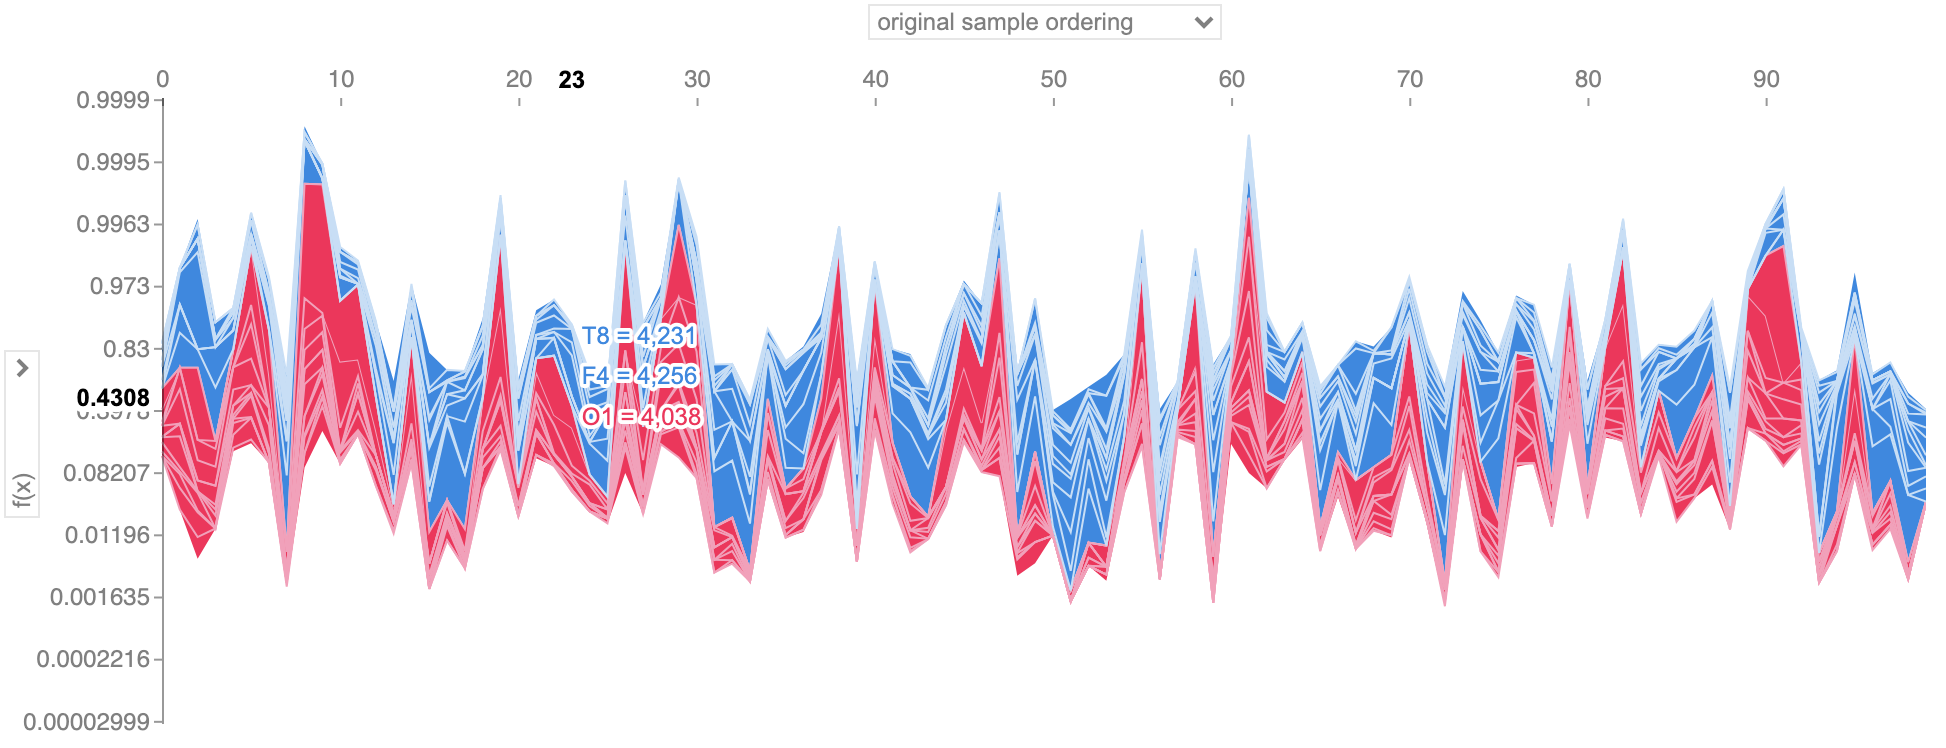
\includegraphics[width=\linewidth]{shap_timeseries.png}

\end{frame}

\begin{frame}{Как сделать лучше?}

    \begin{itemize}
        \item В качестве признаков на текущем моменте брать несколько состояний предыдущих моментов
        \item Использовать RNN и считать hidden state некоторым ''суперпризнаком''
        \item Для нахождения нетривиальных зависимостей можно использовать графовые нейросети
    \end{itemize}
\end{frame}


\begin{frame}{Задачи seq2label}

    \centering
    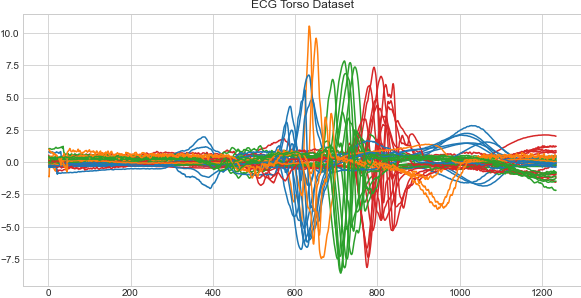
\includegraphics[width=0.7\linewidth]{all_classes.png}

    \begin{itemize}
        \item Рассмотрим задачу seq2label (распознавание человека по его ЭКГ)
        \item Разделим временной ряд на равные кусочки и будем считать их ''суперпризнаками''
        \item Выключение ''суперпризнака'' $=$ замена на среднее/шум
    \end{itemize}

\end{frame}

\begin{frame}{Задачи seq2label: 15 slices}

    \centering
    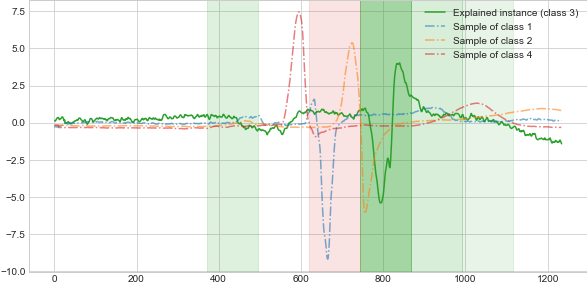
\includegraphics[width=\linewidth]{line_for_3_class_10_slices.png}

\end{frame}

\begin{frame}{Задачи seq2label: 5 slices}

    \centering
    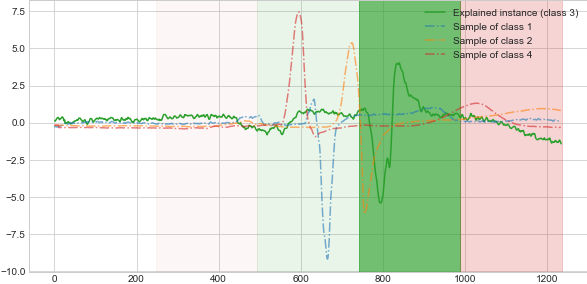
\includegraphics[width=\linewidth]{line_for_3_class_5_slices.png}

\end{frame}


\begin{frame}{Задачи seq2label: 25 slices}

    \centering
    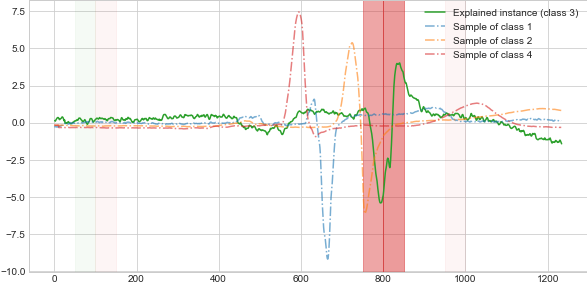
\includegraphics[width=\linewidth]{line_for_3_class_25_slices.png}

\end{frame}


\begin{frame}{Дальнейшие исследования}

    \begin{itemize}
        \item Сверточные нейронные сети
        \item Графовые нейронные сети
        \item Реккурентные нейронные сети
        \item Использование SHAP вместо LIME для задачи seq2label
    \end{itemize}
\end{frame}

\begin{frame}
    \LARGE Спасибо за внимание!
\end{frame}

\begin{frame}{Библиография}
    \begin{enumerate}  
        \item Christoph Molnar. Interpretable Machine Learning.
        \item Lundberg S. M., Lee S. I. A unified approach to interpreting model predictions – 2017. – С. 4768-4777.
        \item Ribeiro M. T., Singh S., Guestrin C. ''Why should i trust you?'' Explaining the predictions of any classifier – 2016. – С. 1135-1144.
        \item  André Ferreira. Interpreting recurrent neural networks on multivariate time series
        \item CinCECGtorso
        \item  EEG Eye Blinking Prediction
    \end{enumerate}
\end{frame}


\end{document}